\documentclass{article}

%-------------------------%
% PREAMBUŁA --------------%
%-------------------------%
\usepackage[utf8]{inputenc}
\usepackage[OT4]{polski}
\usepackage{caption}
\usepackage{amsmath}
\usepackage{tikz}
\usepackage{subcaption}
\usepackage{tabularx}
\usepackage{caption}
\usepackage{array}
\usepackage{hyperref}
\usepackage{graphicx}
\usepackage{fancyhdr}
\usepackage[justification=centering]{caption}
\usepackage[margin=60pt]{geometry}
\usepackage{longtable}



%\usepackage[T1]{fontenc}
%\usepackage{amsthm}
%\theoremstyle{plain}
%\usepackage{enumitem}
%\captionsetup[table]{skip=-4pt}
%\usepackage{tabulary}
%\usepackage{sidecap}
%\usepackage{gensymb}
%\usepackage{wrapfig}
%\usepackage{lastpage}
%\usepackage{gensymb}
%\usepackage{lipsum}
%\pagestyle{fancy}


\newlength{\RoundedBoxWidth}
\newsavebox{\GrayRoundedBox}
\newenvironment{GrayBox}[1][\dimexpr\textwidth-4.5ex]%
   {\setlength{\RoundedBoxWidth}{\dimexpr#1}
    \begin{lrbox}{\GrayRoundedBox}
       \begin{minipage}{\RoundedBoxWidth}}%
   {   \end{minipage}
    \end{lrbox}
    \begin{center}
    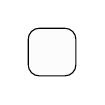
\begin{tikzpicture}%
       \draw node[draw=black,fill=black!1,rounded corners,%
             inner sep=2ex,text width=\RoundedBoxWidth]%
             {\usebox{\GrayRoundedBox}};
    \end{tikzpicture}
    \end{center}}

%------- Typy kolumn do ustawiania szerokości ------- %
\newcolumntype{L}[1]{>{\raggedright\let\newline\\\arraybackslash\hspace{0pt}}m{#1}}
\newcolumntype{C}[1]{>{\centering\let\newline\\\arraybackslash\hspace{0pt}}m{#1}}
\newcolumntype{R}[1]{>{\raggedleft\let\newline\\\arraybackslash\hspace{0pt}}m{#1}}








\begin{document}

%-------------------------%
%Tabela nagłówkowa -------%
%-------------------------%

\begin{table}[h]
\begin{tabular}{|l|l|l|l|l|l|}
\hline
\begin{tabular}[c]{@{}l@{}}
Wydział:\\ WFiIS\end{tabular} &
\multicolumn{2}{l|}{\begin{tabular}[c]{@{}l@{}}
Imię i nazwisko:\\ 1. Axel Zuziak\\ 2. Marcin Węglarz \end{tabular}} 
& Rok \textbf{II}         
& Grupa \textbf{B}          
& Zespół \textbf{03}      \\ \hline
\textbf{\begin{tabular}[c]{@{}l@{}}
LABOLATORIUM\\ TECHNIK \\ JĄDROWYCH\end{tabular}} &
\multicolumn{4}{l|}{ Temat:\textbf{ Statystyczny charakter rozpadów promieniotwórczych.}
	 }                                                                                                                       & \multicolumn{1}{c|}{\begin{tabular}[c]{@{}c@{}}
Nr ćwiczenia\\ \textbf{1+9}
\end{tabular}} \\ \hline
\begin{tabular}[c]{@{}c@{}}
Data wykonania:\\ 04.03.2015
\end{tabular} &
\begin{tabular}[c]{@{}c@{}}
 Data oddania:\\ 18.03.2015
\end{tabular} &
\begin{tabular}[c]{@{}c@{}}
Zwrot do poprawy: \\ 
\end{tabular}                                 
& 
\begin{tabular}[c]{@{}c@{}}
Data oddania: \\ 
\end{tabular}&
\begin{tabular}[c]{@{}c@{}}
Data zaliczenia:\\
\end{tabular}& 
\begin{tabular}[c]{@{}c@{}}
OCENA:\\
\end{tabular}       
\\ & & & & & \\ \hline
\end{tabular}
\end{table}
%-----Koniec tabeli------

%%%%%%%%%%%% Wstęp %%%%%%%%%%%%
\section{Cel ćwiczenia}
Celem ćwiczenia jest wyznaczenie zawartości procentowej wodoru w badanej próbce metodą neutronową. Przybliżenie zagadnienia detekcji neutronów oraz ich oddziaływania z materią.
\section{Wstęp teoretyczny}
Ideą ćwiczenia jest wykorzystanie faktu, że wodór jest wyjątkowo dobrym spowalniaczem neutronów (neutrony tracą przy zderzeniu centralnym prawie 100\% swojej energii kinetycznej), ze względu na zbliżone masy atomu wodoru oraz neutronu. Jeżeli na próbke będą padały jedynie neutrony prędkie to strumień neutronów termicznych po przejściu przez próbkę będzie proporcjonalny do gęstości atomów wodoru w badanym materiale. \\

Jako źródło neutronów wykorzystuję się źródło Pu-Be, gdzie pluton jest emiterem cząstek alfa, 
które następnie ulegają reakcji z jądrami berylu, który ma niską energię separacji neutronu.\\
\[^9_4\text{Be }(\alpha,n)\ ^{12}_6\text{C}\]
Neutrony powstałe w powyższej reakcji mają różne prędkości, natomiast w doświadczeniu potrzebny jest jedynie strumień neutronów prędkich. W tym celu pomiędzy źródłem a badaną próbką umieszcza się osłonę kadmową. Kadm wykazuję szczególnie duży przekrój czynny na absorpcję neutronów termicznych i przekrój ten gwałtownie maleje dla wyższych energii, dzięki czemu pełni ona rolę filtra przepuszczającego jedynie neutrony o większej energii.\\\\
Kolejnym celem na drodze strumienia neutronów jest już badana próbka. Jak wspomniano powyżej wodór ze względu na praktycznie identyczną masę z masą neutronu bardzo wydajnie je spowalnia. W praktyce większość neutronów spowolnionych przez próbkę jest wynikiem ich oddziaływania z jądrami wodoru, dzięki czemu możemy szukać korelacji pomiędzy ilością zliczeń neutronów termicznych w detektorze, a gęstościa wodoru w badanej próbce (ponieważ przekrój czynny na oddziaływanie neutronów z jądrami wodoru w głównej mierze zależy od jego gęstości). \\\\
Przed przystąpieniem do wyznaczania nieznanej zawartości wodoru należy wyznaczyć prostą korelacji częstości zliczeń od znanej zawartości wodoru w próbkach wzorcowych. W tym celu do punktów pochodzących z próbek wzorcowych wystarczy dopasować prostą na przykład metodą najmniejszych kwadratów.\\\\
W końcu po przejściu przez próbkę neutrony wpadają do detektora. W doświadczeniu jako detektora użyto licznika proporcjonalnego z dodatkiem gazowego BF$_3$.




\section{Aparatura i wykonanie ćwiczenia}
\begin{itemize}
	\item \textbf{Neutronowy miernik wodoru}
	\item \textbf{Wzmacniacz impulsowy}
	\item \textbf{Zasilacz wysokiego napięcia}
	\item \textbf{Analizator amplitudy}
	\item \textbf{Przelicznik}
\end{itemize}

Ćwiczenie rozpoczęto od zapoznania się z aparaturą pomiarową. Przed przystąpieniem do wykonywania pomiarów zmierzono wszystkie wymiary geometryczne zarówno próbek wzorcowych: $W1,W2,...W7$ jak i tych, dla których wyznaczano gęstość wodoru: $P1,P2,...P7$. Zanotowano wagi poszczególnych próbek. Wykonano pomiary przy pomocy neutronowego miernika wodoru dla wszystkich próbek.

\section{Wyniki pomiarów i obliczenia.}

\subsection{Wyznaczenie objętości i gęstości badanych próbek.}
Przy pomocy linijki zmierzono wymiary geometryczne badanych próbek. Wyniki pomiarów i obliczeń przedstawiono w tabeli \ref{wynikiW}.

\begin{table}[h!]
\centering
\label{wynikiW}
\caption{Wymiary geometryczne próbek wzorcowych.}
\begin{tabular}{|C{2cm}|C{2cm}|C{2cm}|C{2cm}|}\hline
	Próbka & Waga [g] & Objętość [cm$^3$] & Zawartość $H$ [\%] \\ \hline
		W7	&	298,4	&	346,40	&	15,1 \\ \hline
		W6	&	436,25	&	361,28	&	8,89 \\ \hline
		W5	&	414,5	&	345,58	&	8,08 \\ \hline
		W4	&	478,44	&	338,70	&	6,42 \\ \hline
		W3	&	538,28	&	346,40	&	5,45 \\ \hline
		W2	&	434,46	&	337,72	&	2,05 \\ \hline
		W1	&	766,3	&	361,28	&	0 \\ \hline

\end{tabular}
\end{table}

\begin{table}[h!]
\centering
\label{wynikiP}
\caption{Wymiary geometryczne badanych próbek}
\begin{tabular}{|C{2cm}|C{2cm}|C{2cm}|C{2cm}|}\hline
	Próbka & Waga [g] & Objętość V [cm$^3$] & U(V) [cm$^3$] \\ \hline
		P1	&	181,31	&	331,89	&	10,14 \\ \hline
		P2	&	371,6	&	345,58	&	10,46  \\ \hline
		P3	&	511,34	&	345,58	&	10,46 \\ \hline
		P4	&	590,2	&	310,37	&	9,78 \\ \hline
		P5	&	593,58	&	338,70	&	10,30 \\ \hline
		P6	&	416,6	&	346,40	&	10,40 \\ \hline
		P7	&	439,47	&	361,28	&	10,67 \\ \hline

\end{tabular}

\end{table}
\newpage
\subsection{Cechowanie neutronowego miernika wodoru}
Do otrzymanych wyników (tabela \ref{cechowanie_tab}) dopasowano prostą metodą regresji korzystając z programu Gnuplot:
\begin{equation}
	J = a_0 + a_1\rho_H
\end{equation}
 Otrzymano wartości:
 \begin{equation*}
 	a_1 = 43,0112 \pm 1,451\cdot 10^4
 \end{equation*}
 \begin{equation*}
 	a_0 = 9487,86 \pm 1273
 \end{equation*}
Zatem otrzymana krzywa cechowania przyjmuje postać:
\begin{equation*}
	J = 430112\rho_H + 9487,86
\end{equation*}



\begin{figure}[h!]
	\fontsize{6}{8}\selectfont % zmniejszam czcionke
	\centering
	\resizebox{1.0\textwidth}{!}{% GNUPLOT: LaTeX picture with Postscript
\begingroup
  \makeatletter
  \providecommand\color[2][]{%
    \GenericError{(gnuplot) \space\space\space\@spaces}{%
      Package color not loaded in conjunction with
      terminal option `colourtext'%
    }{See the gnuplot documentation for explanation.%
    }{Either use 'blacktext' in gnuplot or load the package
      color.sty in LaTeX.}%
    \renewcommand\color[2][]{}%
  }%
  \providecommand\includegraphics[2][]{%
    \GenericError{(gnuplot) \space\space\space\@spaces}{%
      Package graphicx or graphics not loaded%
    }{See the gnuplot documentation for explanation.%
    }{The gnuplot epslatex terminal needs graphicx.sty or graphics.sty.}%
    \renewcommand\includegraphics[2][]{}%
  }%
  \providecommand\rotatebox[2]{#2}%
  \@ifundefined{ifGPcolor}{%
    \newif\ifGPcolor
    \GPcolortrue
  }{}%
  \@ifundefined{ifGPblacktext}{%
    \newif\ifGPblacktext
    \GPblacktextfalse
  }{}%
  % define a \g@addto@macro without @ in the name:
  \let\gplgaddtomacro\g@addto@macro
  % define empty templates for all commands taking text:
  \gdef\gplbacktext{}%
  \gdef\gplfronttext{}%
  \makeatother
  \ifGPblacktext
    % no textcolor at all
    \def\colorrgb#1{}%
    \def\colorgray#1{}%
  \else
    % gray or color?
    \ifGPcolor
      \def\colorrgb#1{\color[rgb]{#1}}%
      \def\colorgray#1{\color[gray]{#1}}%
      \expandafter\def\csname LTw\endcsname{\color{white}}%
      \expandafter\def\csname LTb\endcsname{\color{black}}%
      \expandafter\def\csname LTa\endcsname{\color{black}}%
      \expandafter\def\csname LT0\endcsname{\color[rgb]{1,0,0}}%
      \expandafter\def\csname LT1\endcsname{\color[rgb]{0,1,0}}%
      \expandafter\def\csname LT2\endcsname{\color[rgb]{0,0,1}}%
      \expandafter\def\csname LT3\endcsname{\color[rgb]{1,0,1}}%
      \expandafter\def\csname LT4\endcsname{\color[rgb]{0,1,1}}%
      \expandafter\def\csname LT5\endcsname{\color[rgb]{1,1,0}}%
      \expandafter\def\csname LT6\endcsname{\color[rgb]{0,0,0}}%
      \expandafter\def\csname LT7\endcsname{\color[rgb]{1,0.3,0}}%
      \expandafter\def\csname LT8\endcsname{\color[rgb]{0.5,0.5,0.5}}%
    \else
      % gray
      \def\colorrgb#1{\color{black}}%
      \def\colorgray#1{\color[gray]{#1}}%
      \expandafter\def\csname LTw\endcsname{\color{white}}%
      \expandafter\def\csname LTb\endcsname{\color{black}}%
      \expandafter\def\csname LTa\endcsname{\color{black}}%
      \expandafter\def\csname LT0\endcsname{\color{black}}%
      \expandafter\def\csname LT1\endcsname{\color{black}}%
      \expandafter\def\csname LT2\endcsname{\color{black}}%
      \expandafter\def\csname LT3\endcsname{\color{black}}%
      \expandafter\def\csname LT4\endcsname{\color{black}}%
      \expandafter\def\csname LT5\endcsname{\color{black}}%
      \expandafter\def\csname LT6\endcsname{\color{black}}%
      \expandafter\def\csname LT7\endcsname{\color{black}}%
      \expandafter\def\csname LT8\endcsname{\color{black}}%
    \fi
  \fi
  \setlength{\unitlength}{0.0500bp}%
  \begin{picture}(7370.00,5102.00)%
    \gplgaddtomacro\gplbacktext{%
      \csname LTb\endcsname%
      \put(1078,704){\makebox(0,0)[r]{\strut{}$0$}}%
      \csname LTb\endcsname%
      \put(1078,1294){\makebox(0,0)[r]{\strut{}$10000$}}%
      \csname LTb\endcsname%
      \put(1078,1885){\makebox(0,0)[r]{\strut{}$20000$}}%
      \csname LTb\endcsname%
      \put(1078,2475){\makebox(0,0)[r]{\strut{}$30000$}}%
      \csname LTb\endcsname%
      \put(1078,3066){\makebox(0,0)[r]{\strut{}$40000$}}%
      \csname LTb\endcsname%
      \put(1078,3656){\makebox(0,0)[r]{\strut{}$50000$}}%
      \csname LTb\endcsname%
      \put(1078,4247){\makebox(0,0)[r]{\strut{}$60000$}}%
      \csname LTb\endcsname%
      \put(1078,4837){\makebox(0,0)[r]{\strut{}$70000$}}%
      \csname LTb\endcsname%
      \put(1210,484){\makebox(0,0){\strut{}$0$}}%
      \csname LTb\endcsname%
      \put(2033,484){\makebox(0,0){\strut{}$0.02$}}%
      \csname LTb\endcsname%
      \put(2857,484){\makebox(0,0){\strut{}$0.04$}}%
      \csname LTb\endcsname%
      \put(3680,484){\makebox(0,0){\strut{}$0.06$}}%
      \csname LTb\endcsname%
      \put(4503,484){\makebox(0,0){\strut{}$0.08$}}%
      \csname LTb\endcsname%
      \put(5326,484){\makebox(0,0){\strut{}$0.1$}}%
      \csname LTb\endcsname%
      \put(6150,484){\makebox(0,0){\strut{}$0.12$}}%
      \csname LTb\endcsname%
      \put(6973,484){\makebox(0,0){\strut{}$0.14$}}%
      \put(176,2770){\rotatebox{-270}{\makebox(0,0){\strut{}Liczba zliczeń J}}}%
      \put(4091,154){\makebox(0,0){\strut{}Gęstość wodoru w próbce wzorcowej $
ho_H$ [g/cm$^3$]}}%
    }%
    \gplgaddtomacro\gplfronttext{%
      \csname LTb\endcsname%
      \put(5986,4664){\makebox(0,0)[r]{\strut{}$ J = 430112\rho_H + 9487,86$}}%
    }%
    \gplbacktext
    \put(0,0){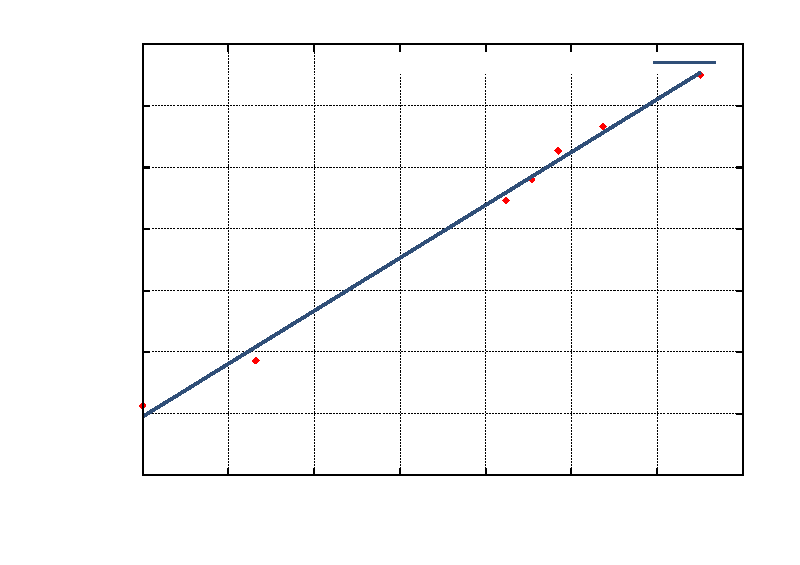
\includegraphics{cechowanie}}%
    \gplfronttext
  \end{picture}%
\endgroup
}	
	\caption{Krzywa cechowania neutronowego miernika wodoru}
	\label{krzywa}
\end{figure}


%%%%%%%%%%%% BIBLIOGRAFIA %%%%%%%%%%%%
\newpage
\begin{thebibliography}{9}
	
	
	\bibitem{1}
	\url{http://nucleardata.nuclear.lu.se/toi/}

	
	\bibitem{DzK}
	B. Dziunikowski, S.J. Kalita
	\emph{Ćwiczenia laboratoryjne z jądrowych metod pomiarowcyh}, Wydawnictwa AGH, Kraków 1995
	
	\bibitem{przybycien}
	Mariusz Przybycień \emph{Tablice Statystyczne}, dostęp on-line\\
	\url{http://home.agh.edu.pl/~mariuszp/wfiis_stat/tablice_ps_wir.pdf}
\end{thebibliography}
\vspace{2cm}








\end{document}





%\textsc{http://nucleardata.nuclear.lu.se/toi/}
%do bibliografii






